\documentclass{article}
\usepackage[utf8]{inputenc}
\usepackage[english]{babel}
\usepackage{graphicx}
\usepackage{float}
\usepackage{listings}
\usepackage{hyperref}
\usepackage{amsmath}
\hypersetup{
    colorlinks=true,
    linkcolor=blue,
    filecolor=magenta,      
    urlcolor=cyan,
}
\urlstyle{same}

\title{Manual 2 - 2do Torneo de Programación Competitiva}
\author{Lions R.C.}
\date{Junio 2019}

\begin{document}

\maketitle

\tableofcontents

\begin{figure}[H]
    \centering
    
\includegraphics[width=0.2\paperwidth]{newblack}
\end{figure}

\section{Estructuras de datos sencillos}

Muchas veces, nos encontramos en medio de un problema que ocupa el uso de algo mas flexible que un arreglo. Si queremos borrar datos de un arreglo, tendriamos que desplazar todos los demás datos que estan enfrente hacia atras, y nuestros resultados se vuelven mas ineficientes o más complicados.

Una solución es utilizar otros estructuras de datos, que almacenan y manejan datos de distintas maneras. En esta sección, solo se explicaran algunas de las muchas estructuras de datos, y la siguiente semana se darán a conocer los demás.

\subsection{Vectores}

Un vector no es nada más que un arreglo dinámico. Esto significa que el vector no tiene un tamaño fijo y puedes agregar y quitar elementos sin problema.

Para crear un vector, es necesario agregar una libreria especifico a esta estructura, llamado \textbf{vector}.

Para incluir esta libreria, se debe de escribir \textbf{\lstinline{\#include <vector>}} en las primeras lineas de tu programa.

\begin{lstlisting}[language=C++, caption=Vectores]
#include <iostream>
#include <vector>

using namespace std;

int main() {

}
\end{lstlisting}

Como un vector se parece a un arreglo, debes definir el tipo de dato que se almacenará a la hora de declararlo. Se puede declarar el vector con el sintaxis \textbf{\lstinline{vector<dato> nombre;}} Como se puede observar, el vector no requiere que le des un tamaño predeterminado.

\begin{lstlisting}[language=C++, caption=Vectores]
#include <iostream>
#include <vector>

using namespace std;

int main() {
    vector<int> enteros;
}
\end{lstlisting}

Aqui se ha declarado un vector de enteros, y para agregarle elementos a este vector, se debe escribir el nombre del vector seguido por un punto y la función \textbf{\lstinline{push_back()}} con el valor del entero entre los paréntesis.

\begin{lstlisting}[language=C++, caption=Agregando valores]
#include <iostream>
#include <vector>

using namespace std;

int main() {
    vector<int> enteros;
    enteros.push_back(1);
    enteros.push_back(4);
    enteros.push_back(9);
}
\end{lstlisting}

Aqui, nuestro vector tendrá los valores de 1, 4 y 9 guardados.

Para ver o modificar el valor en algún indice, se puede utilizar el mismo sintaxis de un arreglo. Si en el ejemplo queremos cambiar el 9 a 7, podemos modificarlo y ver sus cambios con el siguiente código:

\begin{lstlisting}[language=C++, caption=Modificando valores]
#include <iostream>
#include <vector>

using namespace std;

int main() {
    vector<int> enteros;
    enteros.push_back(1);
    enteros.push_back(4);
    enteros.push_back(9);
    for(int i = 0; i < 3; i++) {
        cout << enteros[i] << endl;
    }
    enteros[2] = 7;
    for(int i = 0; i < 3; i++) {
        cout << enteros[i] << endl;
    }
}
\end{lstlisting}

Primero se imprimiran los valores de 1, 4 y 9, luego se verán los valores 1, 4 y 7 en la consola.

Existen mas funciones de los vectores que son utiles, como \textbf{\lstinline{insert()}} que inserta elementos en ciertos indices, \textbf{\lstinline{erase}} que elimina ciertos elementos, \textbf{\lstinline{clear()}} que borra todos los datos en un vector, \textbf{\lstinline{pop_back()}} que elimina el último valor y finalmente \textbf{\lstinline{size()}}, que indica el tamaño de un vector.

\begin{lstlisting}[language=C++, caption=Jugando con vectores]
#include <iostream>
#include <vector>

using namespace std;

int main() {
    vector<int> enteros;
    for(int i = 0; i < 10; i++) {
        enteros.push_back(i);
    }
    enteros.insert(enteros.begin() + 5, 25);
    enteros.erase(enteros.begin() + 7);
    cout << "Cantidad: " << enteros.size() << endl;
    for(int i = 0; i < enteros.size(); i++) {
        cout << enteros[i] << endl;
    }
    enteros.clear();
    cout << "Cantidad: " << enteros.size() << endl;
}
\end{lstlisting}
\href{https://repl.it/@Jamesscn/Juego-de-Vectores}{Liga al código}

Como se puede ver en el código de arriba, se crea un vector de enteros y se llena de los valores de 0 a 9, luego se inserta el valor 25 en el índice 5 y se elimina el valor en el índice 7. Luego se imprime el tamaño del arreglo (12 en ese momento), se imprimen todos los valores, se limpia el vector y finalmente se imprime el tamaño final (cero porque se limpió).

Se debe notar que para las funciones \textbf{insert} y \textbf{erase}, se ocupa llamar a la función begin para ese vector y luego se debe sumar el índice a ese valor. Esta suma luego determina el lugar en la memoria donde esta guardado el valor con ese índice.

\subsection{Pares}

A veces es conveniente guardar cosas en pares, por ejemplo se pueden guardar dos enteros en un par para representar las coordenadas \textbf{x} y \textbf{y} de un plano, o se puede guardar un caracter con un booleano indicando si es vocal. Se puede crear pares de cualquier tipo de dato y los dos tipos no tienen que ser iguales.

Para crear un par, se debe incluir la libreria \textbf{utility} y para declararlo se tiene que escribir \textbf{\lstinline{pair<tipo, tipo> nombre;}}

\begin{lstlisting}[language=C++, caption=Declarando pares]
#include <iostream>
#include <utility>

using namespace std;

int main() {
    pair<int, float> miPar;
}
\end{lstlisting}

Para declarar, se puede utilizar la función \textbf{\lstinline{make_pair}} y ver los datos de este par, se puede llamar el elemento \textbf{first} para el primer dato (en este caso el entero) y \textbf{second} para el segundo dato.

\begin{lstlisting}[language=C++, caption=Declarando pares]
#include <iostream>
#include <utility>

using namespace std;

int main() {
    pair<int, float> miPar;
    miPar = make_pair(20, 4.472136);
    cout << miPar.first << " " << miPar.second << endl;
}
\end{lstlisting}

Combinado con arreglos o vectores, pueden servir para una multitud de aplicaciones. Digamos que queremos guardar todos los puntos de un triángulo en un plano para verlos después. Podemos guardar un arreglo de tres pares correspondientes a los tres puntos de ese triángulo:

\begin{lstlisting}[language=C++, caption=Arreglo de pares]
#include <iostream>
#include <utility>

using namespace std;

int main() {
    pair<int, int> triangulo[3];
    for(int i = 0; i < 3; i++) {
        int x, y;
        cin >> x >> y; //Lee las coordenadas
        pair<int, int> punto = make_pair(x, y);
        triangulo[i] = punto;
    }
}
\end{lstlisting}

Como se puede ver en el código, primero leemos dos números de la consola tres veces, correspondiendo a las X y las Y de los puntos del triángulo. Luego guardamos estos valores en el par \textbf{punto}, donde el primer valor es la X y el segundo valor es la Y. Finalmente, guardamos ese par en el arreglo triángulo.

\subsection{Mapas}

El mapa es una estructura de datos bastante util debido a que mapea un valor a otro, como indicaría el nombre. Esto te permite asociar algún valor con otro para su busqueda rápida. Puedes declarar un mapa incluyendo la libreria \textbf{map} y escribiendo \textbf{\lstinline{map<tipo, tipo> nombre;}}

Digamos que quieres guardar las edades de cada uno de tus amigos. Una manera de hacer esto es tener un arreglo de pares con el nombre de tu amigo y su edad, y luego para obtener la edad de alguno de ellos tendrías que iterar sobre todos tus amigos hasta encontrar el que quieres. Una alternativa más fácil es usar un mapa que simplemente recibe el nombre de tu amigo y que te da su edad.

Les mostraremos las dos opciones, empezando con la implementación de este problema con un arreglo de pares:

\begin{lstlisting}[language=C++, caption=Implementación con pares]
#include <iostream>
#include <utility>

using namespace std;

int main() {
    int n;
    cin >> n; //Lee el numero de amigos
    pair<string, int> edades[n];
    //Guardar todos los amigos y sus edades
    for(int i = 0; i < n; i++) {
        string nombre;
        int edad;
        cin >> nombre >> edad;
        pair<string, int> amigo = make_pair(nombre, edad);
        edades[i] = amigo;
    }
    //Buscar el amigo "Juan" y desplegar su edad
    for(int i = 0; i < n; i++) {
        if(edades[i].first == "Juan") {
            cout << "Juan tiene " << edades[i].second << endl;
            break;
        }
    }
}
\end{lstlisting}

Como se puede ver, se guardaron todos los valores en un arreglo de pares y luego se tuvo que hacer una busqueda de todos los amigos hasta encontrar a Juan. Esta es la simplificación con map:

\begin{lstlisting}[language=C++, caption=Implementación con map]
#include <iostream>
#include <map>

using namespace std;

int main() {
    int n;
    cin >> n; //Lee el numero de amigos
    map<string, int> edades;
    for(int i = 0; i < n; i++) {
        string nombre;
        int edad;
        cin >> nombre >> edad;
        edades[nombre] = edad;
    }
    //Buscar el amigo "Juan" y desplegar su edad
    cout << "Juan tiene " << edades["Juan"] << endl;
}
\end{lstlisting}

Como se puede ver, el primer valor funciona como un estilo de índice que guarda el segundo valor, y se puede utilizar cualquier tipo de variable como este índice.

Pero tambien se debe aclarar que hay dos tipos de mapa, el mapa ordenado y el mapa desordenado. Hasta ahorita, hemos estado utilizando el mapa ordenado o \textbf{map}. El mapa desordenado se llama \textbf{\lstinline{unordered_map}} y para utilizarlo debes incluir la libreria con este mismo nombre.

Existen varias ventajas de usar un mapa desordenado sobre uno ordenado, tiendes a poder modificar y acesar datos mas rapido en un mapa desordenado, pero a la vez ocupa mas memoria que un mapa ordenado. También tiene el mismo sintaxis.

\begin{lstlisting}[language=C++, caption=Mapa desordenado]
#include <iostream>
#include <unordered_map>

using namespace std;

int main() {
    int n;
    cin >> n; //Lee el numero de amigos
    unordered_map<string, int> edades;
    for(int i = 0; i < n; i++) {
        string nombre;
        int edad;
        cin >> nombre >> edad;
        edades[nombre] = edad;
    }
    //Buscar el amigo "Juan" y desplegar su edad
    cout << "Juan tiene " << edades["Juan"] << endl;
}
\end{lstlisting}

\subsection{Sets}

Sets son como vectores pero con condiciones mas estrictos; Un set no puede tener valores repetidos y no permite la modificación de estos valores. Para utilizar un set, se debe incluir la libreria \textbf{set} y se puede declarar con \textbf{\lstinline{set<tipo> nombre;}}

Para insertar valores en un set, es necesario utilizar la función \textbf{\lstinline{insert()}}. Si se llama insert para un valor que ya existe dentro del set no pasa nada, simplemente es ignorado. Para checar si algun valor es miembro de un set, se puede llamar \textbf{\lstinline{count()}} sobre ese elemento y retornará 0 si no existe o 1 si sí existe.

El siguiente código lee varios números de la consola y luego checa si 25 es uno de ellos.

\begin{lstlisting}[language=C++, caption=Sets]
#include <iostream>
#include <set>

using namespace std;

int main() {
    int n;
    cin >> n;
    set<int> entradas;
    for(int i = 0; i < n; i++) {
        int x;
        cin >> x;
        entradas.insert(x);
    }
    if(entradas.count(25) == 0) {
        cout << "25 no es miembro de este set" << endl;
    } else {
        cout << "25 si es miembro de este set" << endl;
    }
}
\end{lstlisting}

Igual que map, el set tiene una version desordenada llamado \textbf{\lstinline{unordered_set}} que tiene acesos más rapidos a costo de más memoria.

\section{Complejidad de tiempo}

Ningun curso de programación con algoritmos esta completo sin el tema de complejidad de tiempo. Este concepto es fundamental para poder hacer buenos programas, y es lo que permite a un programador resolver problemas de la manera más optima.

Vamos a analizar un programa que obtiene todos los números primos menores a N. Se sabe que un número M es primo siempre y cuando es solo divisible entre 1 y M. Para comprobar que M es primo, podemos hacer un ciclo for que itera de 2 a M - 1 y checa si M es divisible entre cualquiera de estos números. En caso que si es divisible, sabemos que el número no puede ser primo y lo marcamos como un número compuesto.

Esta sería la implementación:

\begin{lstlisting}[language=C++, caption=Probando si M es primo]
#include <iostream>

using namespace std;

int main() {
    int m;
    cin >> m;
    bool primo = true; //Asumimos que es primo hasta encontrar un divisor
    for(int i = 2; i < m; i++) {
        if(m % i == 0) {
            primo = false; //M no es primo
        }
    }
    if(primo) {
        cout << m << " es primo" << endl;
    } else {
        cout << m << " no es primo" << endl;
    }
}
\end{lstlisting}

Si pruebas este código con números mayores o iguales a dos indicará si es o no es primo. Ahora queremos probar si todos los números de 2 a N son primos, y podemos encerrar este código en otro ciclo for:

\begin{lstlisting}[language=C++, caption=Encontrando primos menores que N]
#include <iostream>

using namespace std;

int main() {
    int n;
    cin >> n;
    for(int m = 2; m < n; m++) {
        bool primo = true; //Asumimos que es primo hasta encontrar un divisor
        for(int i = 2; i < m; i++) {
            if(m % i == 0) {
                primo = false; //M no es primo
            }
        }
        if(primo) {
            cout << m << endl;
        }
    }
}
\end{lstlisting}

Al correr este código se debera de imprimir una lista de primos después de darle el número N. Pero si se usa N = 100,000 o 1,000,000 se puede notar que el código se tarda algunos segundos en completar, y entre más grande es N, más se tarda.

Nosotros queremos optimizar este código para que pueda encontrar todos los números primos menores a 1,000,000 en muy poco tiempo. Analizando el problema, se te ocurre imprimir 2, iniciar M en 3 en lugar de 2 y saltar en incrementos de 2 para asegurar que M siempre es impar, ya que el único primo par es 2. Al saltar en incrementos de dos, solo checaras si la mitad de los números son primos y razonas que esto debe ser dos veces más rapido porque eliminas la mitad de los pruebas. Asi queda la implementación:

\begin{lstlisting}[language=C++, caption=¿Optimizando?]
#include <iostream>

using namespace std;

int main() {
    int n;
    cin >> n;
    cout << 2 << endl;
    for(int m = 3; m < n; m += 2) {
        bool primo = true; //Asumimos que es primo hasta encontrar un divisor
        for(int i = 2; i < m; i++) {
            if(m % i == 0) {
                primo = false; //M no es primo
            }
        }
        if(primo) {
            cout << m << endl;
        }
    }
}
\end{lstlisting}
\href{https://repl.it/@Jamesscn/Programa-ineficiente}{Liga al código}

Corres este programa y notas que imprime lo mismo que el programa anterior, pero tambien notas que dura practicamente lo mismo que el programa anterior tambien. ¿Por qué sera que al no probar la mitad de los números, el tiempo no se reduce a la mitad, si no que dura practicamente lo mismo?

Esto puede ser explicado con complejidades de tiempo.

\subsection{Número de operaciones}

Vamos a analizar el código anterior de los números primos. Imaginemonos que cada operación se tarda un nanosegundo en hacerse y que cada línea de código (sin incluir ciclos y funciones) cuenta como una operación. Si queremos contar el número de operaciones que nuestro programa hace cada vez que se ejecuta, podemos analizarlo línea por línea y obtener una expresión matemática.

Vamos a considerar que el programa inicia justo después de leer la entrada de N de la consóla y vamos a denotar X como el número de operaciones. Podemos ver que en la siguiente línea se llama cout, asi que podemos decir que X = 1 hasta ahorita. Luego, se ingresa en el primer ciclo, que corre (N - 3) / 2 veces. En cada uno de estos ciclos, se hace una operación que declara primo como cierto, luego se corre otro ciclo for. Sabemos que el segundo ciclo for corre M - 2 veces, y que consiste de 2 lineas de código, una comparación y una igualación. Luego, se sale de ese ciclo y se hacen dos operaciónes mas, otra comparación y una impresión a la consola.

Fuera del primer ciclo, determinamos que hay una sola operación y el primer ciclo.
Dentro del primer ciclo, se corren 3 lineas de código (la declaración de primo y su comparación para luego imprimir a la consola) y el segundo ciclo.
Dentro del segundo ciclo, Se corren 2 lineas de código.

Podemos ir elaborando una formula mátematica. Si consideramos A como el número de operaciones fuera del primer ciclo, B como el número de operaciones dentro del primer ciclo y C como el número de operaciones dentro del tercer ciclo, obtenemos este sistema de ecuaciones:

\begin{align}
    A &= 1 + \frac{N - 3}{2} * B \\
    B &= 3 + (M - 2) * C \\
    C &= 2
\end{align}

Juntando estas tres ecuaciones, se puede obtener X, las operaciones totales.

\begin{equation}
    X = 1 + \frac{N - 3}{2} * (3 + (M - 2) * 2)
\end{equation}

Esta ecuación no esta muy bonita y puede ser confusa. Como no nos interesa saber la cantidad exacta de operaciones, sino que un aproximado, podemos simplificar esta formula quitando algunas partes. Sabemos que este número sera algo muy grande si incrementamos N, asi que podemos ignorar las partes insignificantes.

Primero, se puede quitar el 1 que suma $\frac{N - 3}{2} * (3 + (M - 2) * 2)$ debido a que cuando N es muy grande, no nos va a importar. Luego, se puede quitar el 3 que suma $(M - 2) * 2$ porque tambien se volvera insignificante cuando M es muy grande. Tambien quitaremos el 3 que resta N y el 2 que resta M para obtener la siguiente expresión:

\begin{equation}
    X \approx \frac{N}{2} * (M * 2)
\end{equation}

Esta formula es muchisimo más practico, y puede simplificado aún mas para dar que $X \approx N * M$. Si volvemos a repetir todo el proceso con nuestro programa anterior que sumaba de uno en uno, llegaremos al mismo resultado.

\begin{equation}
    X \approx N * M
\end{equation}

\subsection{Límites}

Nos conviene expresar el tiempo de ejecución de nuestras programas como una especie de función que depende de las entradas, porque asi podemos darnos una idea de como va a comportar a la hora de recibir entradas grandes. Digamos que comparamos dos programas A y B que calculan lo mismo, y el primero tiene una ecuación de operaciones $X = N$ y el segundo tiene otra ecuación $X = N^2$. Si comparamos las gráficas de ambas funciones, nos damos cuenta que el tiempo de ejecución de B aumenta a una velocidad más rapida que el tiempo de ejecución de A.

\begin{figure}[H]
    \centering
    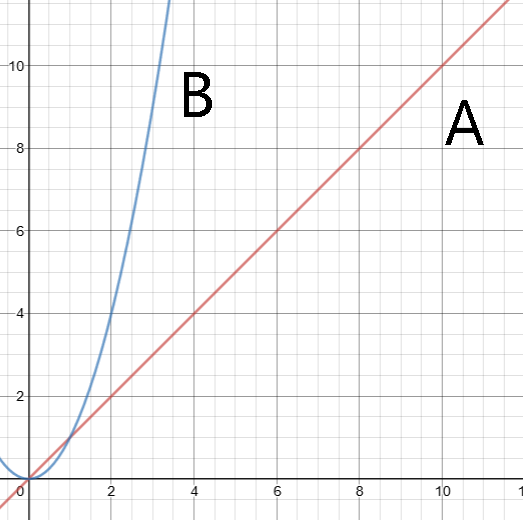
\includegraphics[width=0.3\paperwidth]{nsquared}
\end{figure}

Esto significa que si le damos una entrada de aproximadamente 1,000,000 a A y a B, ¡A podría tardar un segundo mientras que B podría tardar 12 dias! Es muchisimo mas conveniente tener la respuesta de un problema en un segundo que tener que esperar varios dias.

Pero esto es en el peor de los casos, en el mejor de los casos, se les puede dar una entrada de 1 y ambos programas terminan instantaneamente. Por esa rázon, se tiende a pensar en el peor de los casos.

Estas expresiones que hemos estado obteniendo se llaman los complejidades de tiempo de A y B, y existen maneras faciles de determinar cual es el complejidad de tiempo de un algoritmo. Al peor de los casos se le denota con la letra O, y se tiende a encerrar su expresión entre parentesis. Por ejemplo, podemos decir que A tiene \textbf{O(N)} mientras que B tiene \textbf{O($N^2$)}.

La manera mas facil de determinar el complejidad de tiempo de un algoritmo es dividirlo en secciones de ciclos y sumar estos terminos, y descartar todo lo que no sea el termino más grande. Si tenemos un programa con un solo ciclo que se repite N veces, se puede decir que tiene complejidad \textbf{O(N)} porque lo que esta dentro de ese ciclo se repite N veces. Si hay dos ciclos anidados que se repiten N veces, tiene complejidad \textbf{O($N^2$)} porque se multiplica las N iteraciones del primer ciclo con las N iteraciones del segundo. Ahora se mostrará el ejemplo de dos ciclos separados que se repiten N veces:

\begin{lstlisting}[language=C++, caption=Encontrando primos menores que N]
#include <iostream>

using namespace std;

int main() {
    int n;
    cin >> n;
    cout << "Los numeros de 0 a N - 1:" << endl;
    for(int i = 0; i < n; i++) {
        cout << i << endl;
    }
    cout << "Los numeros pero ahora al reves:" << endl;
    for(int i = n - 1; i >= 0; i--) {
        cout << i << endl;
    }
}
\end{lstlisting}

El complejidad del ambos ciclos es O(N) y si se deciden sumar resultarían en la expresión O(2N), pero como el complejidad es una representación de la escala de tiempo que se abarca en un programa, el dos es innecesario y se deberia de quitar para dar O(N) denuevo. Esto significa que si se tienen 2, 3 o incluso más ciclos for que se estan sumando aqui, no tendrán un impacto grande en el tiempo de ejecución.

Si se decide combinar un ciclo de O($N$) con un ciclo de O($N^2$), al sumar los terminos se obtendría O($N^2 + N$). Como $N^2$ es el termino mas significante, cuando se vuelve muy grande N se hará insignificante y no tendrá un gran impacto en el programa. Por esa razón, se debe quitar la N de esa suma para dar O($N^2$).

Esto significa que sin importar que existen otros ciclos en el programa, el tiempo de ejecución siempre será proporcional a la sección mas lenta del programa. Si se tiene un programa sencillo sin ciclos se puede determinar que este es de tamaño O(1) o es de tiempo constante, lo que significa que siempre se tardará el mismo tiempo sin importar el tamaño de N.

Con esto, podemos explicar la razón por la que no funcionaba nuestro programa que calculaba primos y podemos encontrar una manera de hacerlo más eficiente.

\begin{lstlisting}[language=C++, caption=¿Optimizando?]
#include <iostream>

using namespace std;

int main() {
    int n;
    cin >> n;
    cout << 2 << endl;
    for(int m = 3; m < n; m += 2) {
        bool primo = true; //Asumimos que es primo hasta encontrar un divisor
        for(int i = 2; i < m; i++) {
            if(m % i == 0) {
                primo = false; //M no es primo
            }
        }
        if(primo) {
            cout << m << endl;
        }
    }
}
\end{lstlisting}

Como podemos ver, hay un ciclo con complejidad O(N/2) y hay otro adentro de él con complejidad O(M). Como se quitan las coeficientes a los complejidades, el primer ciclo tendrá complejidad O(N). Al multiplicar los dos complejidades, se obtiene que el programa es de complejidad O($N * M$). En el peor de los casos, $M = N$ asi que podemos sustituir M por N para obtener que nuestro programa tiene O($N^2$). Si queremos mejorar nuestro programa, debemos cambiar las Ns por terminos mas pequeños. No podemos quitar la primera N o el primer ciclo porque es la que imprimirá que números son primos, asi que debemos buscar modificar el segundo ciclo. En este, estamos iterando de 2 a M - 1 para ver si un valor es divisible entre M.

Una propiedad de los números que no son primos es que todos sus divisores estan en pares excepto la raíz cuadrada en caso de que sea un número cuadrático. Asi que si no se han encontrado pares hasta llegar a la raíz de un número, se puede determinar que ese número no tiene divisores después de su raiz cuadrada y entonces debe ser primo. Esto nos dice que podemos reducir nuestra busqueda de divisores de 2 hasta la raiz cuadrada de M.

\begin{lstlisting}[language=C++, caption=¿Optimizando?]
#include <iostream>
#include <cmath>

using namespace std;

int main() {
    int n;
    cin >> n;
    cout << 2 << endl;
    for(int m = 3; m < n; m += 2) {
        bool primo = true; //Asumimos que es primo hasta encontrar un divisor
        for(int i = 2; i <= sqrt(m); i++) {
            if(m % i == 0) {
                primo = false; //M no es primo
                break;
            }
        }
        if(primo) {
            cout << m << endl;
        }
    }
}
\end{lstlisting}

Con esta optimización, podemos determinar que nuestro programa tendra complejidad O($N * \sqrt{M}$). Como $M = N$ en el peor de los casos, nuestro complejidad termina siendo O($N \sqrt{N}$). Si comparamos las gráficas de O($N^2$), O($N \sqrt{N}$) y O($N$), podemos ver que O($N \sqrt{N}$) queda justo en medio, por lo que significa que es más rapido que nuestra ultima solución O($N^2$) pero no tán rapido como O($N$).

\begin{figure}[H]
    \centering
    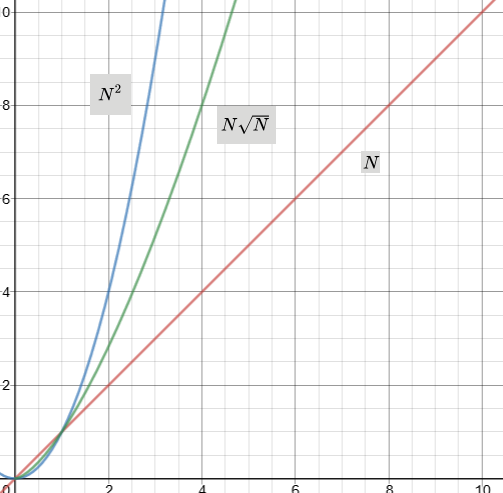
\includegraphics[width=0.3\paperwidth]{nsquaredn}
\end{figure}

Si corremos el código, podemos ver una mejora enorme.

\end{document}